\chapter{Imágenes radiográficas y mejora de contraste} % Título del capítulo
\label{Chapter2}
\lhead{Capítulo 2. \emph{Imágenes radiográficas y mejora de contraste}}

Este capítulo presenta los fundamentos del dominio del problema: las características de las imágenes radiográficas y en particular de las ortopantomografías, las técnicas de mejora de contraste basadas en ecualización de histograma, y las métricas objetivas empleadas para evaluar la calidad de una imagen mejorada.

\section{Imágenes radiográficas digitales}

Una radiografía digital es una representación bidimensional de la atenuación que sufren los rayos X al atravesar los tejidos del paciente. Cada píxel almacena un nivel de intensidad proporcional a la densidad radiológica acumulada a lo largo del rayo correspondiente; en imágenes de 8 bits, estos niveles se cuantifican en el rango $[0, 255]$. Los tejidos de alta densidad, como el hueso y el esmalte dental, absorben mayor radiación y aparecen en tonos claros (radiopacos), mientras que los tejidos blandos y las cavidades aparecen en tonos oscuros (radiolúcidos).

La calidad diagnóstica de una radiografía depende principalmente de tres factores \citep{Gonzalez2018}:

\begin{itemize}
    \item \textbf{Contraste:} diferencia de intensidad entre estructuras adyacentes. Un contraste insuficiente impide distinguir tejidos con densidades similares.
    \item \textbf{Nitidez:} definición de los bordes de las estructuras anatómicas.
    \item \textbf{Ruido:} variaciones aleatorias de intensidad que no corresponden a estructuras reales, inherentes al proceso de adquisición.
\end{itemize}

En la práctica clínica, factores como la dosis de radiación (que se procura minimizar), la calibración del equipo, el posicionamiento del paciente y las características anatómicas individuales producen imágenes con problemas de contraste: subexposición, sobreexposición, rango dinámico comprimido o histogramas sesgados hacia los extremos de la escala de grises.

\section{Ortopantomografía}

La ortopantomografía o radiografía panorámica dental es una técnica radiográfica extraoral que produce una única imagen del conjunto maxilofacial: ambos maxilares, la dentadura completa, las articulaciones temporomandibulares y las estructuras adyacentes. Se obtiene mediante un movimiento sincronizado de rotación del tubo de rayos X y del receptor alrededor de la cabeza del paciente.

Sus principales ventajas frente a las radiografías intraorales son la amplitud de la región visualizada, la menor dosis de radiación respecto a un estudio intraoral completo, y la comodidad para el paciente. Se emplea rutinariamente para la evaluación general de la dentición, la planificación de implantes y ortodoncias, la detección de piezas retenidas, quistes, tumores y patologías óseas.

Como contrapartida, la técnica panorámica es particularmente propensa a deficiencias de contraste: la superposición de estructuras, la variación del espesor de los tejidos a lo largo de la trayectoria del barrido y las limitaciones del receptor producen regiones subexpuestas o sobreexpuestas dentro de una misma imagen. Estas deficiencias motivan el uso de técnicas de mejora de contraste \textit{adaptativas}, capaces de realzar localmente cada región de la imagen.

\section{Mejora de contraste basada en histograma}

\subsection{Ecualización de histograma (HE)}

El histograma de una imagen en escala de grises describe la frecuencia de ocurrencia de cada nivel de intensidad. La ecualización de histograma (HE, \textit{Histogram Equalization}) transforma las intensidades mediante la función de distribución acumulada, de modo que el histograma resultante se aproxime a una distribución uniforme y la imagen utilice todo el rango dinámico disponible \citep{Gonzalez2018}.

HE es una transformación global: aplica la misma función de mapeo a todos los píxeles. En imágenes médicas esto resulta problemático, porque regiones con distribuciones de intensidad muy distintas (por ejemplo, hueso denso y tejido blando) reciben la misma transformación, con lo cual el realce beneficia a unas regiones y perjudica a otras, y puede amplificar el ruido de fondo.

\subsection{Ecualización adaptativa (AHE)}

La ecualización adaptativa de histograma (AHE, \textit{Adaptive Histogram Equalization}) \citep{Pizer1987} divide la imagen en regiones contextuales y ecualiza cada una según su histograma local, interpolando las transformaciones entre regiones vecinas para evitar discontinuidades. De este modo el realce se adapta al contenido local. Su principal desventaja es la sobreamplificación del ruido en regiones homogéneas, donde el histograma local se concentra en pocos niveles y la transformación resultante es muy pronunciada.

\subsection{CLAHE}

CLAHE (\textit{Contrast Limited Adaptive Histogram Equalization}) \citep{Zuiderveld1994} extiende AHE incorporando un límite al realce de contraste. Antes de calcular la transformación de cada región contextual, el histograma local se recorta en un umbral (\textit{clip limit}) y el excedente se redistribuye uniformemente entre todos los niveles. Esto acota la pendiente de la función de mapeo y, en consecuencia, la amplificación del ruido.

El comportamiento de CLAHE queda determinado por tres parámetros:

\begin{itemize}
    \item $R_x$: número de regiones contextuales en el eje horizontal.
    \item $R_y$: número de regiones contextuales en el eje vertical.
    \item $C$: límite de recorte (\textit{clip limit}), que controla el realce máximo permitido.
\end{itemize}

Valores pequeños de $R_x \times R_y$ producen un realce casi global; valores grandes intensifican el realce local pero fragmentan la imagen y pueden introducir artefactos. Valores bajos de $C$ producen realces conservadores; valores altos aproximan CLAHE a AHE. La configuración óptima depende del contenido de cada imagen, lo que convierte a la selección de $(R_x, R_y, C)$ en un problema de optimización por imagen \citep{More2015}. La formulación de este problema como optimización multiobjetivo se desarrolla en el Capítulo~\ref{Chapter3}.

La Figura~\ref{fig:clahe_comparacion} compara ambos enfoques sobre una ortopantomografía con contraste degradado. La ecualización global (HE) expande el rango dinámico pero produce un histograma discontinuo en forma de ``peine'' ---nótese que su entropía incluso disminuye respecto a la entrada--- y satura regiones completas de la imagen. CLAHE, en cambio, realza el contraste región por región y produce un histograma continuo con un aumento efectivo de la entropía, preservando la apariencia natural de las estructuras anatómicas.

\begin{figure}[H]
    \centering
    % Figura generada con scripts/generate_clahe_figure.py
    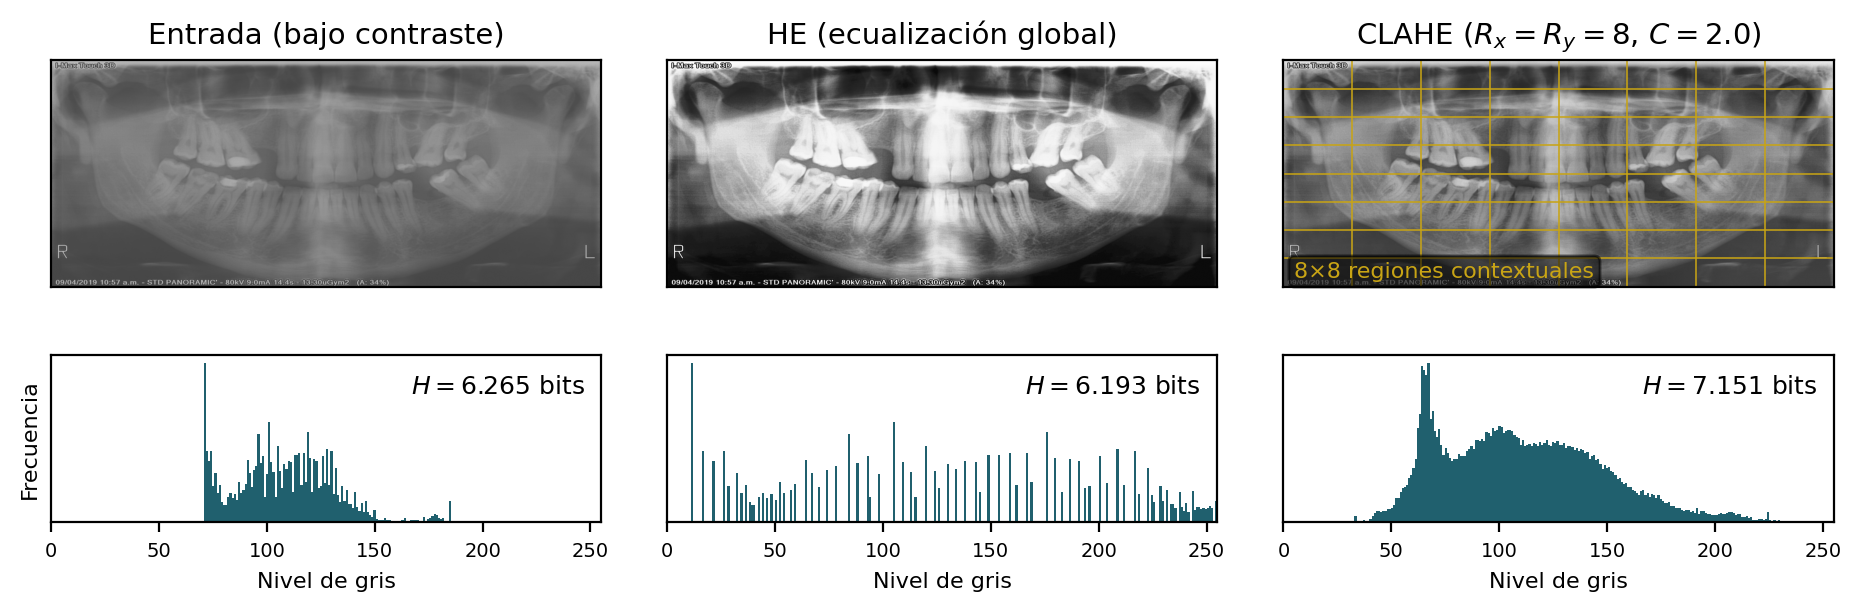
\includegraphics[width=\textwidth]{./Figures/capitulo2/clahe_comparacion}
    \caption[Comparación entre HE y CLAHE sobre una ortopantomografía]{Comparación de técnicas de mejora de contraste sobre una ortopantomografía con bajo contraste (izquierda). La ecualización global HE (centro) expande el rango pero genera un histograma discontinuo y sobresatura regiones, reduciendo incluso la entropía. CLAHE (derecha, con la grilla de $8 \times 8$ regiones contextuales superpuesta) produce un realce local controlado con un histograma continuo y mayor entropía.}
    \label{fig:clahe_comparacion}
\end{figure}

\section{Métricas de evaluación de calidad de imagen}
\label{sec:metricas}

Evaluar si una imagen mejorada es ``mejor'' que la original requiere criterios cuantitativos. Las métricas de calidad de imagen se clasifican en métricas \textit{sin referencia} (evalúan propiedades intrínsecas de la imagen) y métricas \textit{con referencia completa} (comparan la imagen procesada contra una imagen de referencia). El framework propuesto emplea una métrica sin referencia (entropía) y dos métricas con referencia (SSIM y VIF), que capturan aspectos complementarios de la utilidad diagnóstica.

\subsection{Entropía de Shannon}

La entropía \citep{Shannon1948} mide la cantidad de información contenida en la distribución de intensidades de la imagen:

\begin{equation}
H = -\sum_{i=0}^{L-1} p_i \log_2 p_i
\label{eq:entropia}
\end{equation}

donde $L$ es el número de niveles de gris y $p_i$ la probabilidad (frecuencia relativa) del nivel $i$. Una imagen que utiliza pocos niveles de intensidad tiene entropía baja; una imagen con distribución uniforme de intensidades alcanza el máximo $H = \log_2 L$ (8 bits/píxel para $L = 256$). En el contexto de mejora de contraste, una entropía mayor indica un uso más rico del rango dinámico y, potencialmente, mayor cantidad de detalle visible. Es una métrica sin referencia y de tipo beneficio (a maximizar).

\subsection{Índice de similitud estructural (SSIM)}

SSIM (\textit{Structural Similarity Index}) \citep{Wang2004} evalúa la similitud entre dos imágenes $x$ e $y$ combinando tres componentes calculados sobre ventanas locales: luminancia, contraste y estructura:

\begin{equation}
\text{SSIM}(x, y) = \frac{(2\mu_x\mu_y + C_1)(2\sigma_{xy} + C_2)}{(\mu_x^2 + \mu_y^2 + C_1)(\sigma_x^2 + \sigma_y^2 + C_2)}
\label{eq:ssim}
\end{equation}

donde $\mu$, $\sigma^2$ y $\sigma_{xy}$ denotan medias, varianzas y covarianza locales, y $C_1$, $C_2$ son constantes de estabilización. SSIM toma valores en $[-1, 1]$, con 1 para imágenes idénticas. En el framework, SSIM se calcula entre la imagen de entrada y la imagen realzada: actúa como freno estructural, penalizando realces agresivos que distorsionan las estructuras anatómicas. Es una métrica de tipo beneficio.

\subsection{Índice de fidelidad de la información visual (VIF)}

VIF (\textit{Visual Information Fidelity}) \citep{Sheikh2006} cuantifica la fidelidad de una imagen respecto a una referencia desde la perspectiva de la teoría de la información. Modela la imagen de referencia mediante estadísticas de escenas naturales (modelo de mezcla de gaussianas a escala, GSM), el canal de distorsión como una ganancia más ruido aditivo gaussiano, y el sistema visual humano como una fuente adicional de ruido. VIF se define como la razón entre la información mutua que un observador puede extraer de la imagen evaluada y la que puede extraer de la referencia:

\begin{equation}
\text{VIF} = \frac{I(\vec{C}; \vec{F} \mid s)}{I(\vec{C}; \vec{E} \mid s)}
\label{eq:vif}
\end{equation}

donde $\vec{C}$ representa los coeficientes de la referencia, $\vec{E}$ y $\vec{F}$ las versiones percibidas de la referencia y de la imagen evaluada, e $I(\cdot;\cdot)$ la información mutua. En este trabajo se utiliza la versión multiescala en el dominio de píxeles (VIFP) propuesta por los autores.

VIF posee una propiedad singular entre las métricas de calidad con referencia: mientras que SSIM es máximo cuando la imagen evaluada es idéntica a la referencia, VIF puede superar el valor $1$ cuando la imagen evaluada contiene \textit{más} información visual que la referencia, comportamiento típico de un realce de contraste efectivo \citep{Sheikh2006}. Esta propiedad lo hace especialmente adecuado como función objetivo para la mejora de contraste: no penaliza el realce per se, sino la pérdida de información. Además, VIF ha mostrado una correlación alta con el juicio de observadores humanos en estudios de calidad perceptual. Es una métrica de tipo beneficio.

\subsection{Complementariedad de las métricas}

Las tres métricas seleccionadas capturan aspectos distintos y parcialmente en conflicto de la calidad de la imagen mejorada:

\begin{itemize}
    \item La \textbf{entropía} premia el aumento de información en la distribución de intensidades, favoreciendo realces agresivos.
    \item El \textbf{SSIM} premia la preservación estructural respecto a la entrada, favoreciendo realces conservadores.
    \item El \textbf{VIF} premia la fidelidad y ganancia de información visual perceptible, tolerando el realce siempre que no destruya información.
\end{itemize}

Esta tensión entre objetivos es precisamente la que justifica el planteamiento multiobjetivo del problema: no existe una única configuración de CLAHE que maximice simultáneamente las tres métricas, sino un conjunto de soluciones de compromiso que conforman un Frente de Pareto.

\section{Trabajos relacionados}

La sintonización automática de parámetros de CLAHE ha sido abordada mediante diversas metaheurísticas. \citet{More2015} formularon la selección de $(R_x, R_y, C)$ como un problema de optimización multiobjetivo resuelto con SMPSO, empleando la entropía y el SSIM como funciones objetivo sobre radiografías de tórax, y demostraron que las soluciones del Frente de Pareto permiten alcanzar distintos niveles de compromiso entre realce y fidelidad. Este trabajo constituye el antecedente directo del presente framework.

Otros enfoques de la literatura emplean metaheurísticas para la mejora de contraste, ya sea optimizando parámetros de transformaciones de histograma o funciones de mapeo de intensidades directamente; un ejemplo representativo es el uso de algoritmos genéticos para evolucionar la transformación de intensidades guiada por métricas de contraste \citep{Hashemi2010}. Por otra parte, los enfoques basados en aprendizaje profundo dominan actualmente el análisis de imágenes médicas y obtienen resultados destacados también en tareas de realce \citep{Litjens2017}, pero requieren conjuntos de datos de entrenamiento anotados, presentan comportamiento de caja negra y su desempeño depende del dominio de entrenamiento. En contraste, el enfoque de optimización por imagen aquí adoptado no requiere entrenamiento, es interpretable (cada solución es una configuración de parámetros explícita) y es independiente del equipo de adquisición, propiedades relevantes en contextos clínicos con datos escasos y requisitos de trazabilidad.

La contribución diferencial de este trabajo respecto a los antecedentes es doble: (i) la incorporación de VIF como tercera función objetivo, extendiendo el Frente de Pareto a tres dimensiones con una métrica de fidelidad perceptual, y (ii) la integración sistemática de una etapa de decisión multicriterio a posteriori que evalúa ocho métodos MCDM para seleccionar automáticamente la solución final, junto con el análisis de concordancia entre ellos.
